\chapter{Extensions to the Neural Engineering Framework}
\label{chapt:nef-extensions}


\section{Challenges Posed by Neuromorphic Hardware}
\label{sec:challenges}

Apart from having to think differently about how to program.
Some of these are already solved to some extent by standard NEF. Others require more careful consideration / theoretical extensions.

\subsection{Discretization}

\subsection{Quantization}

\subsection{Connectivity}

\subsection{Memory}

Weight factorization on SpiNNaker, Braindrop, and Loihi

\subsection{Spike Traffic}

Amount of internal traffic.

\subsection{External Input-Output}

Amount of external traffic. Also encoding the inputs as spikes, and decoding the outputs.

\subsection{Thermal Variation}

\subsection{Transistor Mismatch}

\subsection{Digital to Analog Conversion}

Pulse-extender

\subsection{Higher-Order Dynamics}

Special case of transistor mismatch


\section{Synaptic Extensions}
\label{sec:synaptic-extensions}

Insert patent here.

\subsection{Linear Transfer Function Characterization}
\label{sec:linear-extensions}

We focus on building a comprehensive theory for linear systems, but many of these same techniques also carry over to the case of nonlinear dynamical systems with heterogeneous synapses~\citep{voelker2017iscas, voelker2017neuromorphic}.

Let $F(s)$ be the transfer function for the linear dynamics that we wish to implement (equations~\ref{eq:lti} and~\ref{eq:ss2tf}), and let $H(s)$ be the transfer function for an arbitrary linear synapse model ($H(s) = \mathcal{L} \left\{ h(t) \right\}$).
As stated in section~\ref{sec:principle3}, introducing the synapse model means replacing the integrator ($s^{-1}$) with $H(s)$.
This is equivalent to replacing $s$ with $H(s)^{-1}$.
Notably, substituting $H(s)$ for the integrator results in the transfer function $F \left( H(s)^{-1} \right)$, which no longer implements the original, desired dynamics $F(s)$. %, via the change-of-variables $s \longleftrightarrow H(s)^{-1}$.
However, we would like to ensure that the new dynamics match the originally specified $F(s)$.
The key insight is that we can determine a new function, $F^H(s)$, such that $F^{H}\left( H(s)^{-1} \right) = F(s)$.
That is, we can solve for a function that provides the original dynamics when implemented using the transfer function $H(s)$ as the dynamical primitive.
This is formalized by the following definition:
\begin{definition} \label{def:maps-onto}
A function $F^{H}(s)$ ``maps $F$ onto $H$'' if and only if it satisfies:
\begin{align} \label{eq:maps-onto}
F^{H}\left( \frac{1}{H(s)} \right) = F(s) \text{.}
\end{align}
\end{definition}

This definition compactly expresses the notion of a ``change of dynamical primitive'', in that $F(s)$ is mapped from the canonical primitive, $s^{-1}$, onto some new primitive, $H(s)$.
Trivially, $F(s)$ maps itself onto $s^{-1}$.
Non-trivial examples are given throughout sections~\ref{sec:lowpass}--\ref{sec:general}.
%To see this, we apply the key insight to some $F^{H}(s)$ to reveal that substituting the integrator for the synapse results in the dynamics $F^{H}(H(s)^{-1})$, which is equal to $F(s)$ if and only if it maps $F$ onto $H$, by definition~\ref{def:maps-onto}.
%Then, to compensate for this change in dynamics, we must solve for some transfer function $F^{H}(s)$ that satisfies definition~\ref{def:maps-onto}.
%This effectively means inverting the change-of-variables $s \longleftrightarrow H(s)^{-1}$.

Once we identify a $F^{H}(s)$ that maps $F$ onto $H$, any state-space model $\left( A^H\text{,}\, B^H\text{,}\, C^H\text{,}\, D^H \right)$ that satisfies
\begin{equation} \label{eq:ss-mapped}
F^{H} \left( s \right) = C^H \left( sI - A^H \right)^{-1}B^H + D^H
\end{equation}
will implement the desired dynamics when using $H(s)$ as the dynamical primitive, by equations~\ref{eq:ss2tf} and~\ref{eq:maps-onto} (see Figure~\ref{fig:lti-system-mapped-general}).

\begin{figure}
  \centering
  \resizebox{\columnwidth}{!} {
	\begin{tikzpicture}[auto, node distance=2cm,>=latex']
	  \node [input, name=input] {};
	  \node [coordinate, name=fanin, right of=input] {};
	  \node [block, right of=fanin, node distance=1.5cm] (B) {$B^H$};
	  \node [sum, right of=B, node distance=2cm] (sum) {$+$};
	  \node [block, right of=sum, node distance=2cm] (integ) {$H(s)$};
	  \node [block, right of=integ, node distance=3.5cm] (C) {$C^H$};
	  \node [sum, right of=C, node distance=2cm] (sumout) {$+$};
	  \node [output, right of=sumout] (output) {};
	
	  \node [block, below of=integ] (A) {$A^H$};
	  \node [block, above of=integ] (D) {$D^H$};
	
	  \draw [-] (input) -- node {$\V{u}$} (fanin);
	  \draw [->] (fanin) -- node {} (B);
	  \draw [->] (fanin) |- (D);
	  \draw [->] (D) -| node {} (sumout);
	  \draw [->] (B) -- node {} (sum);
	  \draw [->] (sum) -- node {} (integ);
	  \draw [->] (integ) -- node [name=fanout] {$\V{x}$} (C);
	  \draw [->] (fanout) |- (A);
	  \draw [->] (A) -| node {} (sum);
	  \draw [->] (C) -- node {} (sumout);
	  \draw [->] (sumout) -- node {$\V{y}$} (output);
	\end{tikzpicture}  
  }
  \caption{ \label{fig:lti-system-mapped-general}
    Block diagram for a LTI system, equivalent to Figure~\ref{fig:lti-system}, with the integrator replaced by a more general linear filter $H(s)$.
    The state-space model $\left( A^H\text{,}\, B^H\text{,}\, C^H\text{,}\, D^H \right)$ is obtained from some transfer function $F^{H}(s)$ that maps $F$ onto $H$, as defined in the text.
    This generalizes Figure~\ref{fig:lti-system-mapped} to arbitrary linear synapse models.
  }
\end{figure}

Therefore, supposing $F^{H}(s)$ satisfies definition~\ref{def:maps-onto}, and that it is convertible to a state-space model (equation~\ref{eq:lti}), then Figure~\ref{fig:lti-system-mapped-general} is just another form of Figure~\ref{fig:lti-system}, but with the integrator replaced by the synapse.
Note that this construction, on its own, does not specify how to find a satisfying $F^{H}(s)$, nor whether such a function exists, nor whether it can be converted to a state-space model.
We provide several examples leading to such a specification in section~\ref{sec:general}.
%This will be made clear through a number of examples, culminating with an approach that recovers an important result from linear systems theory (see appendix~\ref{app:discrete-connection}).
%In appendix~\ref{app:state-space} we discuss our freedom to choose state-space models, and the connection to choice of encoders in the NEF.

Before proceeding, we remark that the above theory directly carries over from the continuous-time domain to the discrete-time domain.
The discrete-time formulation of a LTI system is similar to equation~\ref{eq:lti}, but increments time in steps of length $dt$:
\begin{equation} \label{eq:dlti}
\begin{split}
\V{x}[t+dt] &= \bar{A}\V{x}[t] + \bar{B}\V{u}[t] \text{,} \\
\V{y}[t] &= \bar{C}\V{x}[t] + \bar{D}\V{u}[t] \text{,}
\end{split}
\end{equation}
where the discrete state-space model $\left( \bar{A}\text{,}\, \bar{B}\text{,}\, \bar{C}\text{,}\, \bar{D} \right)$ fully defines the system.
The discrete-time equivalent to the Laplace transform is the $z$\emph{-transform}, named for its use of the variable $z$ to denote the complex frequency domain.
In this domain, $z^{-1}$ plays the role of $s^{-1}$, by performing a discrete shift forwards, one step in time (i.e.,~a delay of one time-step), instead of integration.
A well-known result is that the transfer function of this discrete LTI system---defined as the ratio of the $z$-transform of the output to the $z$-transform of the input---is equal to $F(z) = \bar{C} (zI - \bar{A})^{-1} \bar{B} + \bar{D}$.
Consequently, all of the previous discussion carries over to discrete LTI systems.
In particular, for a discrete synapse expressed using the $z$-transform, $H(z)$, we have the analogous definition:
\begin{definition} \label{def:discrete-maps-onto}
A function $F^{H}(z)$ ``maps $F$ onto $H$'' if and only if it satisfies:
\begin{align} \label{eq:discrete-maps-onto}
F^{H}\left( \frac{1}{H(z)} \right) = F(z) \text{.}
\end{align}
\end{definition}
Given some $F^{H}(z)$ that maps $F$ onto $H$, any state-space model $\left( \bar{A}^H\text{,}\, \bar{B}^H\text{,}\, \bar{C}^H\text{,}\, \bar{D}^H \right)$ that satisfies
\begin{equation} \label{eq:dss-mapped}
F^{H} \left( z \right) = \bar{C}^H \left( zI - \bar{A}^H \right)^{-1}\bar{B}^H + \bar{D}^H
\end{equation}
will implement the desired dynamics $F(z)$ when using $H(z)$ as the dynamical primitive.
Hence, the task of determining $F^{H}(\cdot)$ is identical for both continuous- and discrete-time domains---it is only $F(\cdot)$ and $H(\cdot)$ that differ.

\subsubsection{Continuous Lowpass Synapse}

The first example we consider demonstrates that our new theory recovers the standard form of Principle~3 from the NEF (see section~\ref{sec:principle3}).
For the case of a continuous-time first-order lowpass filter (equation~\ref{eq:lowpass}), $H(s) = \frac{1}{\tau s + 1}$, let:
\begin{align*}
F^H(s) &:= C \left( sI - (\tau A + I) \right)^{-1} \left( \tau B \right) + D \\
&= C \left( \left(\frac{s-1}{\tau}\right)I - A \right)^{-1}B + D \text{.}
\end{align*}
Then, 
\begin{align*}
F^H \left( \tau s + 1 \right) &= C \left( \left(\frac{(\tau s + 1) - 1}{\tau}\right) I - A \right)^{-1}B + D \\
&= F(s)\text{,} 
\end{align*}
which satisfies definition~\ref{def:maps-onto}.
Therefore, by equation~\ref{eq:ss-mapped},
\begin{equation} \label{eq:p3-novel}
\begin{aligned}
A^H &= \tau A + I \text{,} & \quad C^H &= C \text{,} \\
B^H &= \tau B \text{,} & \quad D^H &= D \text{.}
\end{aligned}
\end{equation}
%$A^H = \tau A + I$, $B^H = \tau B$, $C^H = C$, and $D^H = D$.
This completes our novel proof of Principle~3 from section~\ref{sec:principle3}.

\subsubsection{Discrete Lowpass Synapse}

When simulating any NEF network on a digital computer, we necessarily use time-steps of some length $dt > 0$ to advance the state of the network, updating at discrete moments in time~\citep{bekolay2013nengo}.
For instance, Nengo currently uses a default of $dt = 1$\,ms, and implements a zero-order hold~(ZOH) discretization of the synaptic filter.
Implementing ZOH means that all continuous-time signals are held constant within each time-step.
This discretization of equation~\ref{eq:lowpass} gives:
\begin{equation}
H(z) = \frac{1 - a}{z - a} \text{,} \quad a := e^{-\frac{dt}{\tau}} \text{.} \nonumber
\end{equation}
If our desired transfer function is expressed in continuous-time, $F(s)$, then we should also discretize it to $F(z) = \bar{C} (zI - \bar{A})^{-1} \bar{B} + \bar{D}$, with the same time-step, and again using ZOH discretization for consistency.
Let,
\begin{align*}
F^H(z) &:= \bar{C} \left(zI - \frac{1}{1 - a} \left(\bar{A} - aI \right) \right)^{-1} \left( \frac{1}{1-a}\bar{B} \right) + \bar{D} \\
&= \bar{C} \left( \left(z(1 - a) + a \right)I - \bar{A} \right)^{-1}\bar{B} + \bar{D} \text{.}
\end{align*}
Then, 
\begin{align*}
F^H \left( \frac{z-a}{1-a} \right) &= \bar{C}\left( \left( \frac{z-a}{1-a}(1 - a) + a \right)I - \bar{A} \right)^{-1}\bar{B} + \bar{D} \\
&= F(z) \text{,}
\end{align*}
which satisfies definition~\ref{def:discrete-maps-onto}.
Therefore, by equation~\ref{eq:dss-mapped},\begin{equation} \label{eq:discrete-p3}
\begin{aligned}
\bar{A}^H &= \frac{1}{1 - a} \left(\bar{A} - aI\right) \text{,} & \quad \bar{C}^H &= \bar{C} \text{,} \\
\bar{B}^H &= \frac{1}{1-a}\bar{B} \text{,} & \quad \bar{D}^H &= \bar{D} \text{,}
\end{aligned}
\end{equation}
provides an exact implementation of the desired system for digital architectures, regardless of the simulation time-step (assuming ZOH).
% Consequently, we use this method in the simulations reported in this paper unless otherwise noted.

\subsubsection{Delayed Continuous Lowpass Synapse}

Next, we consider a continuous-time first-order lowpass filter with a time-delay of $\lambda$:
\begin{equation} \label{eq:delayed-lowpass}
H(s) = \frac{e^{-\lambda s}}{\tau s + 1} \text{.}
\end{equation}
This same model has been proposed by \citet[][equation~6.2]{roth2009modeling} as a more realistic alternative to equation~\ref{eq:lowpass}, that includes an axonal transmission delay of length $\lambda$ (on the order of $\tau$) to account for the finite-velocity propagation of action potentials.
\TODO{\url{https://en.wikipedia.org/wiki/RC\_time\_constant\#Delay} time-delay is proportional to the square of the wire length}
By commutativity of convolution, modeling the delay in the synapse (as in equation \ref{eq:delayed-lowpass}) is equivalent to modeling the delay in spike propagation.
Equation~\ref{eq:delayed-lowpass} may also be used to account for feedback delays within some broader setting (e.g.,~when the feedback term is computed via some delayed system).

Letting $d := \frac{\lambda}{\tau}e^{\frac{\lambda}{\tau}}$, and $W_0(\cdot)$ denote the principal branch of the Lambert-$W$ function~\citep{corless1996lambertw}, we invert $y := H(s)^{-1}$ as follows:
\begin{align*}
&& y &= \left(\tau s + 1\right) e^{\lambda s} && \\
\iff && \frac{\lambda}{\tau}e^{\frac{\lambda}{\tau}} y &= \left( \lambda s + \frac{\lambda}{\tau} \right) e^{\lambda s + \frac{\lambda}{\tau}} && \\
\iff && W_0(dy) &= \lambda s + \frac{\lambda}{\tau} && \\
\iff && \frac{1}{\lambda} W_0(dy) - \frac{1}{\tau} &= s \text{,} &&
\end{align*}
where the second-last line assumes that $|\eta| < \pi$ and $\lambda \text{Re}\left[ s \right] + \frac{\lambda}{\tau} > - \eta \cot \eta$, where $\eta := \lambda \text{Im}\left[ s \right]$, in order for $\lambda s + \frac{\lambda}{\tau}$ to be within the principal branch~\citep[][equation~4.4]{corless1996lambertw}.\footnote{
A simpler (but only sufficient) condition is $\text{Re} \left[ s \right] \ge -\frac{1}{\tau}$ and $ | \text{Im} \left[ s \right] | < \frac{\pi}{2 \lambda}$.
Thus, it suffices to consider input frequencies $< \frac{1}{4\lambda}$\,Hz.}
Therefore,
\begin{align}
&& F^H(s) &:= F\left( \frac{1}{\lambda} W_0(ds) - \frac{1}{\tau} \right) \label{eq:delayed-lowpass-mapped} && \\
\implies && F^H(H(s)^{-1}) &= F^H(y) = F(s) \text{.} && \nonumber
\end{align}

As a demonstration of how we might use this mapping, suppose the desired transfer function for our system is a time-delay of $\theta$ seconds, $F(s) = e^{-\theta s}$ (equation~\ref{eq:tf-delay}).
In this setting, we are attempting to ``amplify'' a delay of $\lambda$ seconds in the synapse into a system delay of $\theta$ seconds at the network level.
Letting $c := e^{\frac{\theta}{\tau}}$ and $r := \frac{\theta}{\lambda}$, and then substituting $F(s)$ into equation~\ref{eq:delayed-lowpass-mapped}, provides the required function:
\begin{align}
F^H(s) = \exp \left\{ -\theta \left( \frac{1}{\lambda} W_0(ds) - \frac{1}{\tau} \right) \right\} = c \exp \left\{-r W_0(ds) \right\} = c \left( \frac{W_0(ds)}{ds} \right)^r \text{.} \nonumber
\end{align}
This may be numerically converted into a state-space model, of arbitrary dimensionality $q$, via the $\left[q-1/q\right]$ Pad\'e approximants of the following Maclaurin series:
\begin{align} \label{eq:lambert-delay}
F^H(s) = c r \sum_{i=0}^\infty \frac{(i+r)^{i-1}}{i!} (-ds)^i \text{.}
\end{align}
To our knowledge, there is no closed-form expression for the Pad\'e approximants of equation~\ref{eq:lambert-delay}, but there are methods to compute them accurately and in $\bigoh{q^2}$ time~\citep{sidi2003practical}.
Given these approximants, we may follow the same procedure from section~\ref{sec:delay-implementation} to obtain a LTI system in the form of equation~\ref{eq:lti}.
In section~\ref{sec:pure_delay}, we use this approach to improve the accuracy of the delay network demonstrated in section~\ref{sec:delay-implementation}. %(see~Figure~\ref{fig:lambert}).
We remark that each of $d$, $c$, and $r$ are dimensionless (i.e.,~unitless) constants that can be used to relate measurable properties of a biological system that may be governed by this description to the necessary network-level computations.

\subsubsection{General Linear Synapse}

Finally, we consider the general class of all linear synapse models of the form:
\begin{equation} \label{eq:synapse}
H(s) = \frac{1}{\sum_{i=0}^k c_i s^i} \text{,}
\end{equation}
for some polynomial coefficients $\left( c_i \right)$ of arbitrary degree $k$.
To the best of our knowledge, this class includes the majority of linear synapse models used in the literature.
For instance, this includes the first-order lowpass synapse that is standard in the NEF.
It also includes the second-order alpha synapse, $\frac{1}{(\tau s + 1)^2}$~\citep{rall1967distinguishing}---the convolution of two exponentials with identical time-constants---which is commonly used in biological models~\citep{koch1989methods, destexhe1994synthesis, mainen1995reliability, destexhe1998kinetic, roth2009modeling}.
The alpha synapse essentially filters the spike-trains twice, to produce PSCs with finite (non-instantaneous) rise-times.
In addition, equation~\ref{eq:synapse} includes a generalization of the alpha synapse, the double-exponential synapse, $\frac{1}{(\tau_1 s + 1)(\tau_2 s + 1)}$~\citep{wilson1989simulation}---the convolution of two exponentials with time-constants $\tau_1$ and $\tau_2$---which has different rise- and fall-times to account for the separate time scales of rapid transmitter binding followed by slow unbinding~\citep{destexhe1994synthesis, hausser1997estimating, roth2009modeling}.
The double-exponential is also a suitable model to account for parasitic capacitances in neuromorphic hardware~\citep{voelker2017iscas}.
Furthermore, equation~\ref{eq:synapse} includes a higher-order generalization of the alpha synapse, the gamma kernel, $\frac{1}{(\mu^{-1} s + 1)^k}$~\citep[][equation 19]{de1992gamma}. 
Finally, this class contains more exotic models, such as the $Q$-bandpass synapse model, $\frac{1}{\frac{1}{\omega^2}s^2 + \frac{1}{\omega Q}s + 1}$, where $\omega$ is the peak frequency in radians per second, and $Q$ is inversely proportional to the bandwidth.
Such synapses have been used to model bandpass filtering from mechanoreceptors in the fingertip~\citep{voelker2016a} or from rods in the retina~\citep{armstrong2003bandpass}.

As well, in appendix~\ref{app:discrete-connection}, we demonstrate how to use equation~\ref{eq:synapse} to model synapses with pure delays, and to prove a complete connection to ZOH discretization.
%Within the NEF, both the alpha and double-exponential have the advantage of filtering the neural activity twice, thus reducing the spike-noise relative to the first-order lowpass.  CE: just didn't fit well anymore.
Specifically, by the use of Pad\'e approximants, we may rewrite any transfer function with a Taylor series expansion (even those that are irrational or improper) in the form of equation~\ref{eq:synapse}---albeit with some radius of convergence.
This permits us to model, for instance, synapses with pulse-extended responses~\citep{voelker2017iscas}.\footnote{
Pad\'e approximants are computed ``manually'' by \citet[][equations~9--11]{voelker2017iscas} to obtain a second-order approximation in the form of equation~\ref{eq:synapse}.
}
Similarly, the delayed lowpass (equation~\ref{eq:delayed-lowpass}) may be expressed in the form of equation~\ref{eq:synapse}.
% Therefore, equation~\ref{eq:synapse} captures a wide variety of linear postsynaptic responses to some desired degree of accuracy.
Finally, any linear combinations of the aforementioned synapse models will also be a member of this class.
Nonlinear synapse models, such as conductance-based synapses~\citep[e.g.,][equation~6]{destexhe1994efficient}, are a current subject of study in the NEF~\citep{stockel2017}.

%It is interesting to note that although our characterization does not include nonlinear synapse models, such as conductance-based synapses~\citep[][equation~6]{destexhe1994efficient}, recent results indicate that, at least in some common cases, such models may also be accounted for without significantly impacting overall accuracy~\citep{stockel2017}.
%However, these results remain to be thoroughly tested and quantified.

To map $F$ onto equation~\ref{eq:synapse}, we begin by defining our solution to $F^{H}(s)$ in the form of its state-space model (see equation~\ref{eq:ss-mapped}):
\begin{equation} \label{eq:general-linear}
\begin{aligned}
A^H &= \sum_{i=0}^k c_i A^i \text{,} & \quad C^H &= C \text{,} \\
B^H &= \left( \sum_{j=0}^{k-1} s^j \sum_{i=j+1}^k c_i A^{i-j-1} \right) B \text{,} & \quad D^H &= D \text{,}
\end{aligned}
\end{equation}
which we claim satisfies the required identity, $F^{H}(H(s)^{-1}) = F(s)$ (equation~\ref{eq:maps-onto}).
To prove this claim, we first rearrange the following expression:
\begin{align*}
\left( \sum_{j=0}^{k-1} s^j \sum_{i=j+1}^k c_i A^{i-j-1} \right) (sI - A)  &= \sum_{j=0}^{k-1} \sum_{i=j+1}^k s^j c_i A^{i-j-1} (sI - A) \\
&= \sum_{i=0}^{k} \sum_{j=0}^{i-1} s^j c_i A^{i-j-1} (sI - A)  \\
%&= \sum_{i=0}^k c_i (sI - A) \sum_{j=0}^{i-1} s^j A^{i-j-1} \\
&= \sum_{i=0}^k c_i \left( \sum_{j=0}^{i-1} s^{j+1} A^{i - (j + 1)} - s^j A^{i - j} \right) \\
&= \sum_{i=0}^k c_i \left( s^i A^{i - i} - s^0 A^{i-0} \right) \\
&= \left( \sum_{i=0}^k c_i s^i \right) I - \sum_{i=0}^k c_i A^i \\
&= H(s)^{-1}I - A^H \text{.}
\end{align*}
We then complete the proof by substituting this result and the state-space model into our expression for the mapped transfer function from equation~\ref{eq:ss-mapped}:
\begin{align*}
F^H(H(s)^{-1}) &= C^H(H(s)^{-1}I - A^H)^{-1} B^H + D^H \\
&= C(H(s)^{-1}I - A^H)^{-1} \left( \sum_{j=0}^{k-1} s^j \sum_{i=j+1}^k c_i A^{i-j-1} \right) B + D \\
&= C(sI - A)^{-1} B + D \\
&= F(s) \text{.}
\end{align*}
An alternative derivation may also be found in \citet[][section~2.2]{voelker2017neuromorphic}.
An interesting insight gained with this solution is that it is not, in general, the case that $B^H$ is time-invariant, since it depends on $s$.
As a result, solutions will often not be a typical state-space model in the form of equation~\ref{eq:lti}.

Nevertheless, such solutions can still be implemented, as is, in practice.
Since $s^j$ is the $j^{\text{th}}$-order differential operator, this form of $B^H$ states that we must supply the $j^{\text{th}}$-order input derivatives $\V{u}^{(j)}$, for all $j = 1 \ldots k - 1$.
When $k = 1$, as in section~\ref{sec:lowpass}, this is trivial (no derivatives are needed).
For $k > 1$, let us first define $B^H_j:= \left( \sum_{i=j+1}^k c_i A^{i-j-1} \right) B$.
Then equation~\ref{eq:general-linear} shows that the ideal state-space model must implement the input transformation as a linear combination of input derivatives, $\sum_{j=0}^{k-1} B^H_j \V{u}^{(j)}$.
If the derivatives of the input are available to the model, then the $F^{H}(s)$ we described may be used to precisely implement the desired $F(s)$.

However, if the required derivatives are not included in the neural representation, then it is natural to use a ZOH method by assuming $\V{u}^{(j)} = 0$, for all $j = 1 \ldots k - 1$:
\begin{equation} \label{eq:general-linear-approx}
B^H = B^H_0 =  \left( \sum_{i=1}^k c_i A^{i-1} \right) B \text{,}
\end{equation}
with $A^H$, $C^H$, and $D^H$ as before (see equation~\ref{eq:general-linear}).
This is now an equivalent model to equation~\ref{eq:general-linear} assuming ZOH, and in the form of the standard state-space model (equation~\ref{eq:lti}).
In appendix~\ref{app:poles}, we characterize the dynamics of this new system in terms of $F$ and $H$ (independently of the chosen state-space model) for general inputs.
We find that equation~\ref{eq:general-linear-approx} adds $k - 1$ new dimensions, for every dimension in $F$, to the state underlying the resulting dynamical system.
In appendix~\ref{app:discrete-connection}, we show that the our results yield a novel derivation of ZOH discretization for LTI systems.

To our knowledge, this specific state-space architecture has not been explored in theory or in practice.
Given that equation~\ref{eq:general-linear} requires the input derivatives to accurately compute low-dimensional network-level dynamics, this strongly suggests that it is important to represent and compute derivatives in neural systems.
Methods of computing derivatives have been explored by \citet{tripp2010} within the NEF.
As well, it has long been suggested that adaptive neural mechanisms (e.g., synaptic depression or spike-rate adaptation) may also play a fundamental role in computing such derivatives~\citep{abbott2004synaptic, lundstrom2008fractional}.
However, there has typically been less emphasis placed on understanding temporal differentiation in comparison to other temporal operators, such as integration~\citep{tripp2010}.

Finally, we again note that these results translate directly to the discrete-time domain.
The required state-space matrices are the same as in equation~\ref{eq:general-linear}, but with $\left( \bar{c}_i \right)$ corresponding to the coefficients of $H(z)$, bars affixed to each state-space matrix, and $z$ substituted for $s$ in $\bar{B}^H$.
However, the $z^j$ operator is a shift backwards by $j$ time-steps (i.e.,~an acausal lookahead), and so the ZOH assumption is instead $\V{u}[t+j(dt)] = \V{u}[t]$ for all $j = 1 \ldots k - 1$.
Thus, the discrete analog to equation~\ref{eq:general-linear-approx} is:
\begin{equation}
\bar{B}^H = \left( \sum_{j=0}^{k-1} \sum_{i=j+1}^k \bar{c}_i \bar{A}^{i-j-1} \right) \bar{B} \text{.}
\end{equation}

\subsubsection{Relationship to Discretization}

As an aside, there is an interesting connection between definition~\ref{def:maps-onto} and the well-known problem of discretizing a linear dynamical system.
A discrete LTI system (equation~\ref{eq:dlti}) is identical to a continuous LTI system (equation~\ref{eq:lti}), with three adjustments: (1)~the integrator $s^{-1}$ is replaced by a time-delay of $dt$ seconds, (2)~the input signal is sampled every $dt$ seconds, and (3)~the output signal is sampled every $dt$ seconds.
Focusing on point~1, this is precisely the notion captured by definition~\ref{def:maps-onto} with respect to:
\begin{equation*}
H(s) = e^{-(dt)s} = \frac{1}{e^{(dt)s}} = \frac{1}{\sum_{i=0}^\infty \frac{(dt)^i}{i!} s^i} \text{,}
\end{equation*}
by the Maclaurin series of $e^{x}$.
This is in the form of equation~\ref{eq:synapse} with $c_i = \frac{(dt)^i}{i!}$ as $k \rightarrow \infty$.
These coefficients are also the $\left[ 0 / \infty \right]$ Pad\'e approximants of $\sum_{i=0}^\infty \frac{(-dt)^i}{i!} s^i$.

If we make the ZOH assumption---that the input signal is held piecewise-constant over each continuous-time interval of length $dt$---then $\V{u}^{(j)} = 0$ for all $j \ge 1$.
Therefore, by equation~\ref{eq:general-linear-approx}, an equivalent state-space model is:
\begin{align*}
A^H &= \sum_{i=0}^k c_i A^i = \sum_{i=0}^k \frac{\left(A(dt)\right)^i}{i!} = e^{A(dt)} \text{,} & C^H &= C \text{,} \\
B^H &= \left( \sum_{i=1}^k c_i A^{i-1} \right) B = A^{-1} \left(A^H - I\right) B \text{,} & D^H &= D \text{,}
\end{align*}
which is precisely the discrete state-space model $(\bar{A}, \bar{B}, \bar{C}, \bar{D})$ obtained by ZOH discretization.
This follows from the fact that points~2 and~3 coincide with the use of the model from equation~\ref{eq:dlti}.

This connection helps highlight the generality and consistency of our theory.
In particular, the important procedure of discretizing linear state-space models may be viewed as an instance of accounting for changes in dynamical primitives.
Furthermore, as one should hope, the ZOH assumption recovers the correct result, which is normally proven by integrating the linear differential equations over the interval $[0\text{,}\, dt]$.

\subsection{Nonlinear State-Space Characterization}

\subsection{Approximating Derivatives}

Motivated by the theoretical need for driving the synapse with higher-order input derivatives...
Talk about Bryan's paper, and the fact we can approximate the required transfer function $F(s) = s$ or a lowpass filtered version.

\subsubsection{Constant Input Analysis}

Consider the $F^H$ determined by equation~\ref{eq:general-linear-approx}, when the derivatives of the input signal are inaccessible.
Let $\hat{F}(s) := F^{H}(H(s)^{-1})$ be the dynamics of the implemented system for this particular $F^H$.
Due to the ZOH assumption, $\hat{F} \ne F$ in general, and so $F^H$ does not technically map $F$ onto $H$ (see definition~\ref{def:maps-onto}).
As discussed in section~\ref{sec:general}, the approximation only satisfies equation~\ref{eq:maps-onto} when the input is held constant.
To be clear, $\hat{F}(s) = F(s)$ for $s = 0$, but not necessarily for $s \ne 0$.
Thus, it is important to characterize the difference between $\hat{F}$ and $F$ for general inputs.

To do so, we can examine the \emph{poles} of the transfer function $F(s) = \frac{\mathcal{C}(s)}{\mathcal{D}(s)}$, which are defined as the complex roots of $\mathcal{D}(s)$.
The poles of a system fully define the dynamics of its state (up to a change of basis).
For instance, a system is exponentially stable if and only if $\text{Re} \left[ s \right] < 0$ for all poles $s \in \mathbb{C}$.
Furthermore, $s \in \text{sp}(A)$ if and only if $s$ is a pole, where $\text{sp}(A)$ denotes the eigenvalues of the state-space matrix $A$.\footnote{
Note that $\text{sp}(A) = \text{sp}(TAT^{-1})$ for any invertible matrix $T$ with the same shape as $A$.
}
% $\text{sp}(A) = det(sI - A)$
Therefore, we may characterize the poles of $\hat{F}$ in terms of the poles of $F$, in order to understand the behavior of the implemented system.

We begin by deriving the poles of $F^H$, recalling that $A^H = \sum_{i=0}^k c_i A^i$.
Let $\V{v} \ne \V{0}$ be an eigenvector of $A$ with eigenvalue $\lambda$, %(i.e., a pole of $F(s)$),
so that:
\begin{align*}
A\V{v} = \lambda \V{v} \quad \implies \quad A^H \V{v} = \sum_{i=0}^k c_i A^i \V{v} = \left( \sum_{i=0}^k c_i \lambda^i \right) \V{v} \text{.}
\end{align*}
Hence, $\text{sp}\left(A^H \right) = \left\{  \sum_{i=0}^k c_i \lambda^i \,:\, \lambda \in \text{sp}(A) \right\}$ is the full set of eigenvalues for $A^H$.
This is also true for equation~\ref{eq:general-linear}, since $A^H$ is identical, but we do not need this fact.

The denominator of $\hat{F}$ may now be written as $\prod_{\lambda \in \text{sp}(A)} \left( H(s)^{-1} - \sum_{i=0}^k c_i \lambda^i \right)$.
Therefore, the poles of $\hat{F}$ are the roots of the $q$ polynomials:
\begin{equation*}
\mathcal{P}(\phi) := \sum_{i=0}^k c_i \left( \phi^i - \lambda^i \right) \text{,} \quad \lambda \in \text{sp}(A) \text{.}
\end{equation*}
% $H(\phi)^{-1} - \sum_{i=0}^k c_i \lambda^i = 0$, where $\lambda$ is a pole of $F$.
A trivial set of roots are $\phi = \lambda$, and thus each pole of $F$ is also a pole of $\hat{F}$, as desired.
However, for a synapse of order $k$, there will also be $k - 1$ additional poles for every pole of $F$.
For this system to behave as $F$ given low-frequency inputs, we must have the old poles dominate the new poles.
That is, we require $\text{Re} \left[ \lambda \right] \gg \text{Re} \left[ \phi \right]$ for all $\phi \ne \lambda$.

To provide a specific example, let us consider the double-exponential synapse, $H(s)^{-1} = (\tau_1 s + 1)(\tau_2 s + 1)$,
\begin{align*}
\implies && \mathcal{P}(\phi) &= \tau_1 \tau_2 \phi^2 + (\tau_1 + \tau_2) \phi - (\tau_1 \tau_2 \lambda^2 + (\tau_1 + \tau_2) \lambda) = 0 && \\
\iff && \phi &= \frac{-(\tau_1 + \tau_2) \pm \sqrt{(\tau_1 + \tau_2)^2 + 4\tau_1 \tau_2 \left(\tau_1 \tau_2 \lambda^2 + (\tau_1 + \tau_2) \lambda \right)}}{2 \tau_1 \tau_2} && \\
&& &= \frac{-(\tau_1 + \tau_2) \pm \left(2 \tau_1 \tau_2 \lambda + (\tau_1 + \tau_2) \right)}{2 \tau_1 \tau_2} \text{.} &&
\end{align*}
In this instance, the `$+$' case gives back the known poles, $\phi = \lambda$, and the `$-$' case provides the new poles, $\phi = \left(- \frac{\tau_1 + \tau_2}{\tau_1 \tau_2} - \lambda \right)$.
Consequently, the poles of $\hat{F}$ are the poles of $F$, duplicated and reflected horizontally about the real line $- b$, where $b := \frac{\tau_1 + \tau_2}{2 \tau_1 \tau_2}$ (and the imaginary components are unchanged).

Interestingly, $b$ may be rewritten as $\left( \frac{ \tau_1 + \tau_2}{2} \right) / \sqrt{\tau_1^2 \tau_2^2}$, which is the ratio of the arithmetic mean to the geometric mean of $\{\tau_1, \tau_2\}$, which may in turn be interpreted as a cross-entropy expression~\citep{woodhouse2001ratio}.

Regardless, $\hat{F}$ behaves like $F$ when $\text{Re} \left[ \lambda \right] \gg -b$.
For the delay system (equation~\ref{eq:ss-delay}), $\text{Re} \left[ \lambda \right] \propto -\frac{q}{\theta}$ (in fact, the mean value across all $q$ poles achieves equality), and so we need $b \gg \frac{q}{\theta}$.
This predicts that a delay system using the double-exponential synapse, without access to the input's derivative, must necessarily implement a delay that is proportionally longer than $\frac{q}{b}$.
Otherwise, the second-order dynamics from the synapse will dominate the system-level dynamics.
We note that $b^{-1}$ is longest for the case of the alpha synapse ($b^{-1} = \tau$), and shortest for the case of the lowpass synapse ($b^{-1} \rightarrow 0$ as $\tau_2 \rightarrow 0$).



\subsubsection{Taylor-Series Approximation}

\TODO{Include patent method}
...
we considered the alpha synapse:
$$H(s) = \frac{1}{(\tau s + 1)^2} = \frac{1}{\tau^2 s^2 + 2\tau s + 1}$$
and observed that:
$$F' \left( H(s)^{-1} \right) = F(s) \quad \iff \quad F'(s) = F \left( \frac{\sqrt{s} - 1}{\tau} \right) .$$
In general, the final expression, $F \left( \frac{\sqrt{s} - 1}{\tau} \right)$ is not necessarily proper and finite-dimensional (rational in $s$). For instance, with the integrator,
$$F(s) = 1/s \quad \iff \quad F'(s) = \frac{\tau}{\sqrt{s} - 1}$$
is infinite-dimensional (irrational in $s$).
In the patent, we deal with this by taking the Taylor series approximation $(\sqrt{s} - 1) / \tau \approx \left( s - 1 \right) / (2 \tau)$, which yields the approximation: $$F'(s) \approx F \left( \frac{s-1}{2\tau} \right) = \frac{2 \tau}{s - 1} .$$
We can then convert back to the world of $F(s)$ to see what dynamics we've actually implemented:
$$F(s) = F' \left( H(s)^{-1} \right) \approx \frac{2\tau}{(\tau s + 1)^2 - 1} = \frac{2\tau}{\tau s (\tau s + 2)} = \frac{1}{s \left( \frac{\tau}{2} s + 1 \right) } .$$
This reveals that, instead of the integrator, we've implemented an integrator convolved with a lowpass with time-constant $\tau / 2$.

\subsubsection{Lagrange--B\"urmann Approximation}

If the derivatives are not available, but we are okay with changing the state vector, then we may consider making a different approximation.
For instance, in the alpha case, we approximated $F'(s) \approx F \left( \frac{s-1}{2\tau} \right)$ using a first-order Taylor series.
But we could have expanded it out to any order -- this will alter the state and increase the dimensionality of the system.

In general, we are trying to find an $F'(s)$ such that $F'(H(s)^{-1}) = F(s)$.
However, it may not be clear how to do this for general $H(s)^{-1} = \sum_{i=0}^k c_i s^i$, since the inverse of $H(s)^{-1}$ does not necessarily exist.
Fortunately, we can use a powerful tool named the {\it Lagrange--B\"urmann inversion theorem} to approximate the inverse of $H(s)^{-1}$.
Essentially it is a way to get the Taylor series of the inverse of some function around a point without explicitly constructing the inverse. Applying it here around the zero frequency, we have:
\begin{align}
f(s) &:= H(s)^{-1} = \sum_{i=0}^k c_i s^i \nonumber \\
g_n &:= \lim_{s \rightarrow 0} \left[ \frac{\partial^{n-1}}{\partial s^{n-1}} \left( \frac{s}{f(s) - c_0} \right)^n \right] \nonumber \\
F'(s) &\approx F \left( \sum_{n=1}^\infty g_n \frac{(s - c_0)^n}{n!} \right)
\end{align}
in some neighbourhood of $s = 0$.
For some finite truncation of the series $g_n$, this always yields a finite-dimensional and proper approximation of the required $F'(s)$ assuming the same of $F(s)$.
%The resulting dimensionality increases with the order of the approximation.

For example, returning to the alpha example, we have:
\begin{align*}
f(s) &= (\tau s + 1)^2 \\
g_1 &= \lim_{s \rightarrow 0} \left( \frac{s}{ s(\tau^2 s + 2 \tau)} \right) = \frac{1}{2 \tau} \\
\implies F'(s) &\approx F \left( \frac{s - 1}{2\tau} \right)
\end{align*}
which is identical to beforehand.
More generally, for $H(s)^{-1} = \sum_{i=0}^k c_i s^i$, we have $g_1 = \frac{1}{c_1}$,
\begin{equation}
\implies F'(s) \approx F \left( \frac{s - c_0}{c_1} \right) = C \left( sI - (c_1 A + c_0 I) \right)^{-1} (c_1 B) + D.
\end{equation}
Note this is different from the corollary, because the approximations are of a different nature. Before we were approximating the input as a constant signal (and taking the system into account), while here we are approximating the [inverse of the reciprocal of the] synapse as linear around $s = 0$ (independently of the contents of $F(s)$).

But for the integrator (and the alpha) we showed the two approximations were the same.
In fact, one can easily verify that for $F(s) = s^{-1}$ and for {\it all} $H(s)^{-1} = \sum_{i=0}^k c_i s^i$ the two approximations are identical ($B' = c_1 B$, $A' = c_0 I$).

\subsection{Time-Constant Mismatch}
\label{sec:mismatch}

\subsection{Encoding Filters}

Here we consider ensembles of neurons where the $i^{th}$ neuron has a distinct filter applied to its input current, referred to as an `encoding filter' $h^e_i(t)$, in addition to a distinct filter applied to its output spike train, referred to as a `decoding filter' $h^d_i(t)$. 
By linearity of encoding and decoding, the synapse connecting the $j^{th}$ pre-synaptic neuron to the $i^{th}$ post-synaptic neuron becomes:
\begin{equation} \label{eq:syn-factored}
h_{ij}(t) = (h^e_i \ast h^d_j)(t) .
\end{equation}

If, for example, $h^e_i$ and $h^d_j$ are lowpass filters, then $h_{ij}$ will be the double-exponential synapse. If further  they are identical, then this is the alpha synapse.

This can be interpreted as a generalization of Principle~II from the NEF, which normally supposes $h_{ij}(t) = h(t)$ for all $i$ and $j$ within the same ensemble.
This can be used to model the synaptic heterogeneity that arises in real biological systems, or in neuromorphic hardware resulting from transistor mismatch. 

Furthermore (\ref{eq:syn-factored}) can be interpreted as a factorization of the synapses, analogous to the factorization of connection weights \mbox{$w_{ij} = \V{e}_i \, \cdot \, \V{d}_j$}.
We thus use the term `filter' throughout to distinguish the abstract factors of the synapse from their correspondingly realized synapse.
We will also interpret the tuple $(\V{e}_i, h^e_i)$ as the neuron's `temporal encoder', and $(\V{d}_i, h^d_i)$ as the `temporal decoder'.

To be clear, the input current to the $i^{th}$ neuron is now:
\begin{align}
J_i(t) &= \left( \left[ \V{e}_i \cdot \left( \sum_j ( a_j \ast h^d_j) \, \V{d}_j \right) \right] \ast h^e_i \right)(t) \label{eq:factored} \\
       &= \sum_j w_{ij} (a_j \ast h_{ij})(t) . \label{eq:unfactored}
\end{align}
Importantly (\ref{eq:factored}) is more space- and time-efficient to implement than (\ref{eq:unfactored}) for low-dimensional encoders and decoders, since the inner summation (which is also the decoded vector being represented) does not depend on $i$.

We view such an architecture as approximating functions of the form:
\begin{equation} \label{eq:temporal-function}
\hat{f}(\V{x} \ast \hat{h}^e) \ast \hat{h}^d
\end{equation}
where $\hat{f}$ is an approximation of some desired $f$, and $\hat{h}^e$ and $\hat{h}^d$ are approximations of some desired filters $h^e$ and $h^d$.
This is in contrast to the functions that we normally approximate, $\hat{f}(x) \ast h$, which are strictly less computationally powerful.

In order to solve for the decoders $\V{d}$ which approximate this function, it suffices to explicitly simulate the ensemble on some training signal $\V{x}(t)$, determine the corresponding target signal using (\ref{eq:temporal-function}), and then solve for the linear decoders which minimize the root mean-square-error (RMSE) -- also known as least-squares optimization -- between the two signals as per usual in the NEF.
The simulation involves encoding $\V{x}(t)$ through the encoding filters $h_i^e(t)$ and encoding vectors $\V{e}_i$, simulating the neuron models, and finally applying the decoding filters $h_i^d(t)$ to each spike train.

This technique was used in \citet{voelker2016a} and found to be primarily responsible for the performance of the touch classifier overviewed below.

This section is taken from \citep{voelker2016a}.

Giving robots the ability to classify surface textures requires appropriate sensors and algorithms. Inspired by the biology of human tactile perception, we implement a neurorobotic texture classifier with a recurrent spiking neural network, using a novel semi-supervised approach for classifying dynamic stimuli. Input to the network is supplied by accelerometers mounted on a robotic arm. The sensor data is encoded by a heterogeneous population of neurons, modeled to match the spiking activity of mechanoreceptor cells. This activity is convolved by a hidden layer using bandpass filters to extract nonlinear frequency information from the spike trains. The resulting high-dimensional feature representation is then continuously classified using a neurally implemented support vector machine. We demonstrate that our system classifies 18 metal surface textures scanned in two opposite directions at a constant velocity. %In particular, the system correctly classifies 65.6\% of all 1 second test recordings. 
We also demonstrate that our approach significantly improves upon a baseline model that does not use the described feature extraction. 
This method can be performed in real-time using neuromorphic hardware, and can be extended to other applications that process dynamic stimuli online. 

Humans are remarkably adept at perceiving the environment using their sense of touch. By moving the fingertip across a surface, vibrations give rise to perceptual qualities such as roughness \citep{unger2013physical}, stickiness, and slipperiness \citep{klatzky2013haptic, holliins1993perceptual}. Thus, structural details smaller than 1\,\si{\micro\meter} in different quality grades of silk, paper, and grind metal surfaces can be differentiated \citep{weber2013spatial}.
%, smaller than the distance between specialized mechanoreceptors within the fingertip.
%It is made possible by mechanoreceptors innervating our skin which are sensitive to dynamic stimuli, namely vibrations. These origin from the contact area between skin and texture when moving the finger \citep{weber2013spatial}. 
%The relationship, however, is highly on-linear and complex. In the case of texture classification, the challenge lies within finding distinctive features in these vibration patterns. %The challenge  is to find physical quantities which can be linked to perceptual qualities. 
Our goal is to draw inspiration from nature to give robots the ability to classify surface textures in real-time. This ability can be deployed within systems that need to classify tactile stimuli, such as those employed to automate quality control of textured surfaces. 


Dynamic robotic systems for tactile surface sensing have been developed using various technologies \citep{dahiya2010tactile}. In this context, \textit{tactile} implies the sensors physically touch the textured surface. \textit{Dynamic} refers to robotic setups that perform exploratory movements across the surface to accumulate sensor data. % Sensing technologies - Accelerometers
Accelerometers have been used as dynamic vibration sensors for texture discrimination in %\citep{howe1989sensing} 
\citep{howe1993dynamic}, \citep{giguere2011simple} %(mems acc on flexible probe)
and \citep{sinapov2011vibrotactile}. 
By using only the signal variance of two spatially separated vibration sensors, four different textures could be differentiated in \citep{tada2004sensing}. In addition to variance, Giguere and Dudek \citep{giguere2011simple} utilized mean, skewness, kurtosis and some higher order moments of one accelerometer to differentiate between ten fine and coarse textures. 
Other studies have used multiple exploratory movements to boost classification accuracy. For instance, Sinapov et al. \citep{sinapov2011vibrotactile} used five exploratory movements with varying direction and speed, and analyzed the spectrotemporal features to classify twenty naturalistic fine textures with $80\%$ accuracy. Another study kept executing exploratory movements until at least $80\%$ of the movements indicated a specific texture \citep{jamali2011majority}.


% 2. Data processing and exploratory movement
% Systems using different sensors but interesting in terms of data processing: \citep{oddo2011roughness} SSSA biotact sensor using mems pressure sensing, 

However, only a few groups have developed classifiers using spiking neural networks. A closed perception-action loop was built to classify Braille characters \citep{bologna2013closed}, by supplying pressure sensor array data to {\it leaky integrate-and-fire} (LIF) 
neurons, and then using a naive Bayes classifier to control the scanning velocity. 
Another approach classified ten naturalistic textures with $97\%$ accuracy \citep{rongala2015neuromorphic}, by simulating an Izhikevich neuron in response to an array of four piezoresistive sensors, and analyzing the precise spike timing using spike distance metrics. However, these metrics require offline processing of the entire time window, and therefore cannot be implemented in real-time.

% Jeremy Fishel - Bayesian exploration
Related work has also used {\it Bayesian exploration} to optimize the information supporting various textural \mbox{properties \citep{fishel2012bayesian}}. This model is capable of using a number of exploratory movements to classify $117$ textures with a $95.4\%$ success rate. However, the system requires an offline phase to reduce the input signal to a number of scalar values, making it unsuitable for real-time applications. This reduction could also discard valuable information from the input signal, since it is manually crafted using a finite set of properties motivated by psychophysical studies. 

In contrast, we find it possible to automatically discover the most salient {\it features} from a high-dimensional representation of the input stimulus, %and process this signal to extract 
and classify these features {\it online}.  This is challenging since the relationship between a rapidly time-varying tactile stimulus and its resulting perceptual qualities is highly nonlinear \citep{weber2013spatial}. To make this problem tractable, we translate our biological understanding of tactile perception into an artificial network  of spiking neurons, and then train the desired function. Our approach  % from the mechanoreceptors to the classification result
is implemented entirely within a spiking neural network that can be simulated on low-power neuromorphic hardware. 

%As opposed to \citep{jamali2011majority}, we only use data gathered from one type of exploratory movement at one fixed velocity. 
%

When fingers move across a texture, tiny hills and valleys along its surface rapidly excite various types of static and dynamic {\it mechanoreceptors} \citep{weber2013spatial}. Biomechanical processes within these cells convert the physical forces applied by the stimulus into spike trains. We adapt a mechanoreceptor model by Kim et al. \citep{kim2011does} to simulate this process in a population of spiking neurons.  The nervous system routes the mechanoreceptor responses  through the spinal cord where they are  processed by cuneate neurons \citep{saal2014touch}, which function as feature extractors across this spiking activity   \citep{jorntell2014segregation}. This motivates the inclusion of a {\it hidden layer} in the model  to extract a high-dimensional feature representation. We have designed  this layer to encode frequency bands of the stimulus, since frequency is an important factor in psychophysical experiments involving the differentiation of textures \citep{unger2013physical}. 
The population of cuneate neurons project these features to somatosensory cortex, where an abstract percept of the texture is thought to be formed  \citep{jorntell2014segregation}. Our model  learns the mapping from features to textures using a support vector machine (SVM). These learned weights are embedded  within the connection to a recurrent output layer. To summarize, the network encodes the physical stimulus into spiking activity, maps this activity to extract salient features, and finally decodes the resulting spikes to obtain an online classification. 

To implement this model, we employ  the Neural Engineering Framework (NEF), which  provides a method for mapping functions to a biologically plausible spiking neural network \citep{eliasmith2003a}. %This provides our system with a number of unique advantages that advance the field of robotics. 
These networks can be efficiently simulated on neuromorphic hardware such as SpiNNaker \citep{mundy2015}, resulting in significant energy savings \citep{hasler2013finding}. Simulations are also more efficient than all-to-all connected networks due to the use of factored weight matrices \citep{bekolay2013},  and are generally robust to noise and physical variability due to heterogeneity \citep{hunsberger2014}.

Our method uses the NEF to classify surface textures scanned with a robotic setup. We report performance on a set of 18 metal surface textures. This establishes a novel biologically-inspired system that can be simulated in real-time using neuromorphic hardware.

\subsubsection{Mechanoreceptor Model}

\newcommand{\gammafactor}{\mbox{\it $\Gamma$-factor} (GF)}

The human sense of touch uses free nerve endings and specialized mechanoreceptors to sense vibrations on the skin. The latter are composed of two types: 1) slowly adapting type cells which are sensitive to static stimuli; 2) the so-called rapidly adapting type cells. The slowly adapting cells include Merkel (SA1, static pressure) and Ruffini cells (SA2, skin stretch). The rapidly adapting cells are sensitive to transient events such as vibration. These include Meisser (RA, vibration in the range of 1 to about 60\,Hz) and Pacinian cells (PC, vibrations in the range of 30 to about 700\,Hz) \cite{johansson2009coding}. When the finger moves across a surface texture, the skin is excited by vibration patterns influenced by macro- and microscopic topography of the surface in contact. These cells transform the physical stimulus into spiking patterns.

%% Description of the mechanoreceptor population model%%
To mimic this biological representation, our model encodes the vibrations recorded from multiple accelerometers into the spiking activity of a heterogeneous population of mechanoreceptor neuron models.  Since SA2 cells do not contribute directly to fine textural percepts \cite{weber2013spatial}, we only consider PC,  RA, and SA1 type cells for our model. 

%% Description of the individual receptor principle%%

The mechanoreceptor model by Kim et al. \cite{kim2011does} has been shown to accurately reproduce the spike trains of RA and SA1 type cells on a variety of stimuli.  Following this model, we take the acceleration $u(t)$, and its two derivatives $\dot{u}(t)$, $\ddot{u}(t)$, and separate each of them into positive and negative rectified parts resulting in $6$ signals. % We may interpret $u(t)$ as the applied to the fingertip, since force is proportional to acceleration. 
Since acceleration is directly proportional to the net force, we interpret $u(t)$ as the force applied to the fingertip.
Then $\dot{u}(t)$ and $\ddot{u}(t)$ are the first- and second-order changes in force, respectively.  As shown in \mbox{Fig. \ref{fig:touch-network}}, the rectified signals form 6 inputs, which are weighted and summed to form the current to an adaptive LIF neuron.
%As shown in Fig. \ref{fig:netw_struct}, these 6 signals are weighted and summed to form the input current to an adaptive LIF neuron.

This is equivalent to the neural representation of a $6$-dimensional vector $\V{x}(t)$ in the NEF using (\ref{eq-neuron}). Each encoding vector $\V{e}_i$ corresponds to the $6$ weights that depend on the cell type of the $i^{th}$ neuron. Different weights then reproduce the spiking characteristics of different types of mechanoreceptors.  For the PSC model required by the NEF, we use a lowpass filter with time constant $\tau = 1$\,ms on all mechanoreceptors. We found experimentally that this constant works well to balance the need for smoothing (large $\tau$) with the need to maintain high frequencies in the signal (small $\tau$).  To simplify implementation, differentiation is performed by combining this PSC filter with a highpass filter with the same time constant (Laplace transform $\tau s$). Our model differs from the original model only by  the use of an adaptive LIF model instead of the {\it Mihalas-Niebur} model, and by omitting a saturation filter applied to the current. The adaptive LIF model is used in place of $G[\cdot]$ to obtain a neural model that is simpler than Mihalas-Niebur while still supporting adaptation. We then use (\ref{eq-neuron}) to simulate the spiking activity of each neuron in response to the stimulus.

\begin{figure}[!tbp]
    \centering
    \vspace{-2pt}
    \includegraphics[width=0.49\textwidth]{touch-1}
     
    \caption{\label{fig:touch-network} Architecture of the surface texture classifier. Data from three sensors are encoded in the spiking activity of mechanoreceptor neurons. A hidden layer extracts nonlinear features of these spike trains in the frequency domain by convolution with bandpass filters. A recurrently connected output (feedback arrows omitted) represents the score for each class, smoothed over time. This score vector is linearly decoded from the recurrent layer to find the texture with the largest score. Connection weights and neural parameters  are given by the principles of the NEF.}
\end{figure}

Rather than fitting the parameters of the neurons directly to individual model neurons  as in the original model, we uniformly randomize parameters $\alpha_i$, $\beta_i$, and $\V{e}_i$ of $\numprint{40000}$ neurons (this number was chosen to sufficiently sample the space of parameters), and then select those with the highest \gammafactor{} \cite{jolivet2008benchmark} to canonical PC/RA/SA1 models on a standard test stimulus\footnote{Canonical models and test data were obtained by email correspondence with the authors of \cite{kim2011does}. Although PC type cells were not evaluated by the original study, their model included sample PC parameters.}
The GF compares the number of coincidental spikes within a $\pm 2$\,ms window to the expected value generated by a Poisson process with the same firing rate: $1$ implies a perfect match; $0$ a Poisson process; and $-1$ indicates anti-correlation. We use this particular measure to be consistent with the  prior analysis of the original model. %Thus we assure biological realism of the selected populations. 
The pruned population of mechanoreceptors contains $20/300/200$ neurons ($520$ total)  of type PC/RA/SA1, respectively, to match the distribution within a $2$\,cm$^2$ % should cm be italicized?
surface of contact \cite{johansson2009coding}. % Around $0.5\%$ of the total neurons had a \gammafactor{} exceeding $0.8$ with at least one of the canonical PC/RA/SA models.
The GF of selected neurons range from $0.19$ to $0.99$  with mean $0.49$ across all three types. This is promising considering Kim et al. \cite{kim2011does} found the mean GF between individually fit models and their canonical RA/SA1models to be approximately $0.3$.

The resulting distribution of encoders effectively reflects the sensitivity of each cell to various characteristics of the sensory input. By allowing them to vary randomly, the information content of the population is increased \cite{hunsberger2014}. In particular, the network can further process the $6$-dimensional representation using (\ref{eq-decoder})  while being robust to noise.
This need to exploit individual variability is consistent with the conclusion made by Kim et al. \cite{kim2011does} that heterogeneity in afferent fibers matters when conveying precise timing information about the tactile response.

The fingertip has multiple points of contact while scanning a surface, allowing it to pick up spatial features of the stimulus \cite{weber2013spatial}. The above $6$-dimensional encoding is repeated 3 times (for each sensor in our robotic setup)  to form an $18$-dimensional representation, where the encoding vector for each neuron is tuned to different combinations of dimensions from the different sensors. This further improves robustness to noise by exploiting multiple correlated sources of information. %, and effectively permits the neural representation to exploit any nonlinear interactions between sensors. 
The distribution of encoders could also be controlled to match known spatial characteristics of each cell, but for simplicity we set all encoders to be uniformly distributed across the 3 sensor signals.

\subsubsection{Dynamical Feature Extraction}

Given the spiking activity of the population of mechanoreceptors, we now extract a high-dimensional representation in a hidden layer of neurons,  to capture general features of the stimulus.

The $18$-dimensional input representation ($6$ dimensions $\times$ $3$ sensors) is recovered from the spiking activity of the mechanoreceptor population,  by solving (\ref{eq-decoder}) for a $520 \times 18$ decoder matrix $\V{d}$ ($18$ input dimensions for each of the $520$ mechanoreceptor neurons)  using regularized least squares optimization. The parameters of $\numprint{7200}$ LIF neurons (this number was chosen to sufficiently sample the space of neural parameters per dimension), one for each feature in the hidden layer,  are randomly generated, with encoders constrained to each of the possible $18$ dimensions. This forms a sparse $\numprint{7200} \times 18$ encoder matrix $\V{e}$ such that (\ref{eq-conn}) gives the connection weight matrix from the mechanoreceptor population to the hidden layer. % the sparsity reduces time/space by a factor of 18 -- and the number of neurons in this layer is reduced in section \ref{sec_classifier}.
The hidden layer then represents the same $18$-dimensional input at the current point in time, by having learned the optimal decoding from the spikes of the adaptive mechanoreceptor layer. 

Motivated by the importance of stimulus frequency in psychophysical experiments involving texture \mbox{discrimination \cite{unger2013physical}}, our aim is to extract features that encode information about the frequency of the current stimulus.  The weight matrix transforms the activity independently of time, and is therefore insufficient to extract information about its frequency content. Thus, we provide the $i^{th}$ neuron in the hidden layer with its own PSC filter $h_i(t)$, modeled as a {\it $2^{nd}$ order bandpass} filter with Laplace transform
\begin{equation}
\label{eq-bandpass}
H_i(s) = \frac{1}{\frac{1}{\omega_i^2}s^2 + \frac{1}{\omega_i Q_i}s + 1}
\end{equation}
where $\omega_i$ is the peak frequency in radians per second, and $Q_i$ is inversely proportional to the bandwidth. This filter was chosen because it is the linear filter of lowest order that is capable of isolating particular bands of frequencies. 

Each $\omega_i$ %(or $2 \pi f$, where $f$ is the frequency in Hertz) 
is chosen randomly without examining the input data. Since differentiation is a form of highpass filtering, we expect the higher derivatives to represent higher frequency bands more accurately. Thus $\omega_i$ is chosen between $0 - 250$, $125 - 375$, or $250 - 500$\,Hz, depending on whether the neuron is encoding a dimension from $u(t)$, $\dot{u}(t)$, or $\ddot{u}(t)$, respectively. Frequencies above $500$\,Hz are unnecessary due to the refractory rates of neurons ($2$\,ms). We found that randomizing $Q_i$ between $2 - 50$, regardless of dimension, lead to the best results. 

The spiking activity of each hidden neuron encodes a recovered input dimension convolved with a random bandpass filter (see Fig. \ref{fig:netw_struct}). Decoding the square of a particular filter from this population then yields the power of that filter. More generally, any nonlinear functions of the frequency bands that are supported by the neural basis functions\footnote{Eliasmith and Anderson \cite{eliasmith2003a} characterize this in detail using singular value decomposition on the activity matrix, and show that squaring is accurately supported by LIF tuning curves.} can be used as a feature -- a fact readily exploited in  the following subsection.

\subsubsection{Recurrent Classification}

\newcommand{\outputNeurons}{900}

The final layer of our model is a recurrent output layer,  which classifies the spiking activity of the hidden layer into one of $k$ possible surface textures. The output layer is a population of $\outputNeurons{}$ LIF neurons that represent a $k$-dimensional vector %(using (\ref{eq-neuron}) and (\ref{eq-decoder})) 
encoding a {\it score} for each class. The value of $\outputNeurons{}$ was chosen to be large enough to accurately decode all $k$ dimensions using (\ref{eq-decoder}).

Since the activity of the hidden layer is noisy and high-dimensional, we use scikit-learn (v0.16.1) to train a {\it one-vs-all linear support vector machine} (SVM), from the spikes of the hidden layer, without being prone to overfitting  \cite{pedregosa2011scikit}. Since each of the $k$ classifiers  computes a dot product, together they form a $\numprint{7200} \times k$ decoder matrix $\V{d}$ (one decoding vector for each neuron in the hidden layer)  equivalent to solving (\ref{eq-decoder}) using the SVM maximum margin objective.

A $\numprint{\outputNeurons{}} \times k$ encoder matrix $\V{e}$ (one encoding vector for each neuron in the output layer)  is randomly generated, and (\ref{eq-conn}) provides the weight matrix to the output layer. To determine the resulting classification, we again solve for a $\numprint{\outputNeurons{}} \times k$ decoder matrix $\V{d}$, so that (\ref{eq-decoder}) produces an estimate of the $k$-dimensional score vector. The index of the maximum value yields the classification for the given point in time. 

The population is recurrently connected to itself using (\ref{eq-leaky}) to integrate the scores with a leak term. This smooths the classification over time, with different recurrent lowpass time constants ($\tau_0$) altering the rate of adaptation to new stimuli or the forgetting of old evidence. We use $\tau_0 = 50$\,ms  and \mbox{$\tau = 5$\,ms} for the output layer. The value of $\tau$ matches the default synaptic time-constant in our simulation software, while $\tau_0$ was found to help persist correct classifications over time intervals with insufficient evidence in the signal. 

It is important to note that although the SVM itself is linear, its features are not, due to the neural nonlinearities in the hidden layer. This is mathematically equivalent to using a kernel function given by the LIF tuning curves. %This provides the SVM with a rich set features that are nonlinear in the encoded frequencies%
Thus, the SVM nonlinearly separates the encoded frequency bands using randomly generated neural basis functions.

\subsubsection{Software}

All experiments were run using Nengo (v2.0.1), a Python implementation of the NEF \cite{bekolay2013nengo}. Neurons were configured with default parameters, and the parameters from (\ref{eq-neuron}) were randomly sampled across the default ranges. Nengo automatically learned the decoders and connection weights offline, by optimizing the RMSE of (\ref{eq-decoder}) given randomly sampled $\V{x}(t)$ from the unit hypersphere.

The simulations of (\ref{eq-neuron}) used a timestep of $0.5$\,ms ($2$\,kHz). % ($0.2$ times the data sampling rate). -- data sampling rate has not been mentioned yet
The accelerometer data $u(t)$ was streamed as input to the neural network. The spike train of the output population was read to obtain a classification at each timestep. %We now proceed with details of the architecture in Nengo within the context of the NEF.

Details of the experimental setup may be found in \citet{voelker2016a}.

\subsubsection{Results}

\begin{figure}[!htb]
    \centering
    \vspace{1pt}
    \includegraphics[width=0.4\textwidth]{touch-4}
    \caption{\label{fig:touch-raster} Network activity on a $1$ second test segment from the S2.5 %(face milling, $2.5$\,Rz) 
recording. (Top) Normalized accelerometer data from the three sensors, across an interval of $0.2$ to $0.4$\,s. (Middle) Spike raster of 15 (out of 520) randomly selected mechanoreceptor neurons, over this same time interval. (Bottom) Top 4 scores across the entire $1$\,s segment, obtained by decoding the output population. The network correctly classifies the texture as S2.5 at every timestep after the first $10$\,ms.
}
\end{figure}

\begin{table*}[!htbp]
    \centering
    \vspace{5pt}
    \caption{\label{tab:touch-results} Confusion Matrix for $1$\, Second Test Segments (\%) }
    \renewcommand{\arraystretch}{1.1}  % stretch vertical padding to make the table appear cleaner
    \renewcommand{\tabcolsep}{0.195cm}  % squish horizontal padding to avoid overflowing into margins
    \tiny
\begin{tabular}{ | c c || c c c c c c c c c c c c c c c c c c | } \hline & &  \multicolumn{18}{c|}{\bf Predicted} \\ & & F.55 & F1 & F1.6 & H2.5 & H4 & H8 & L2.5 & L4 & L8 & S2.5 & S4 & S8 & P.55 & P1 & P1.6 & G3 & G6 & G10 \\ \hline \hline \multirow{18}{*} {\rotatebox[origin=c]{90}{\bf Actual}} & F.55 & {\bf 96.7} & 0.8 & 0.0 & 0.0 & 0.0 & 0.0 & 0.8 & 0.0 & 0.0 & 0.0 & 0.0 & 0.0 & 0.0 & 0.0 & 0.0 & 0.8 & 0.0 & 0.8 \\ & F1 & 14.2 & {\bf 55.8} & 8.3 & 0.0 & 0.0 & 0.0 & 0.0 & 0.0 & 0.0 & 0.0 & 0.0 & 0.0 & 0.8 & 9.2 & 0.0 & 4.2 & 1.7 & 5.8 \\ & F1.6 & 4.2 & 0.0 & {\bf 80.0} & 0.0 & 0.0 & 0.0 & 0.8 & 2.5 & 1.7 & 0.0 & 1.7 & 0.0 & 0.0 & 7.5 & 0.0 & 0.8 & 0.0 & 0.8 \\ & H2.5 & 0.8 & 0.0 & 1.7 & {\bf 40.8} & 0.0 & 5.8 & 0.0 & 0.0 & 0.8 & 5.0 & 33.3 & 1.7 & 8.3 & 0.0 & 0.8 & 0.0 & 0.0 & 0.8 \\ & H4 & 0.0 & 0.0 & 0.0 & 0.0 & {\bf 99.2} & 0.0 & 0.0 & 0.0 & 0.0 & 0.0 & 0.0 & 0.0 & 0.8 & 0.0 & 0.0 & 0.0 & 0.0 & 0.0 \\ & H8 & 0.0 & 0.0 & 0.0 & 0.0 & 1.7 & {\bf 68.3} & 0.0 & 0.0 & 1.7 & 1.7 & 9.2 & 1.7 & 10.0 & 1.7 & 0.0 & 0.0 & 0.8 & 3.3 \\ & L2.5 & 4.2 & 0.0 & 4.2 & 0.0 & 0.0 & 0.0 & {\bf 73.3} & 0.8 & 7.5 & 6.7 & 2.5 & 0.0 & 0.0 & 0.0 & 0.0 & 0.8 & 0.0 & 0.0 \\ & L4 & 0.0 & 0.0 & 10.0 & 0.0 & 0.0 & 0.0 & 2.5 & {\bf 60.0} & 0.0 & 0.0 & 25.0 & 0.8 & 0.8 & 0.0 & 0.8 & 0.0 & 0.0 & 0.0 \\ & L8 & 3.3 & 0.0 & 10.8 & 0.0 & 0.0 & 0.8 & 16.7 & 8.3 & {\bf 49.2} & 0.0 & 1.7 & 0.8 & 3.3 & 0.8 & 0.0 & 2.5 & 0.0 & 1.7 \\ & S2.5 & 0.0 & 0.0 & 0.0 & 0.8 & 0.0 & 10.8 & 5.0 & 0.0 & 2.5 & {\bf 67.5} & 0.8 & 0.0 & 5.0 & 0.0 & 0.0 & 6.7 & 0.8 & 0.0 \\ & S4 & 0.0 & 0.0 & 0.8 & 0.0 & 0.0 & 0.0 & 0.0 & 1.7 & 0.8 & 1.7 & {\bf 92.5} & 0.0 & 0.0 & 0.8 & 1.7 & 0.0 & 0.0 & 0.0 \\ & S8 & 0.0 & 0.8 & 0.8 & 0.8 & 0.0 & 9.2 & 1.7 & 0.0 & 0.8 & 14.2 & 17.5 & {\bf 40.0} & 0.8 & 1.7 & 6.7 & 0.0 & 0.0 & 5.0 \\ & P.55 & 0.8 & 0.0 & 0.8 & 0.8 & 0.0 & 7.5 & 0.0 & 0.0 & 0.8 & 0.0 & 2.5 & 0.0 & {\bf 75.0} & 5.8 & 0.0 & 4.2 & 0.0 & 1.7 \\ & P1 & 0.8 & 0.0 & 1.7 & 0.0 & 0.0 & 5.0 & 0.0 & 0.8 & 0.0 & 0.0 & 2.5 & 0.0 & 10.8 & {\bf 55.8} & 0.0 & 6.7 & 0.8 & 15.0 \\ & P1.6 & 0.0 & 0.0 & 0.0 & 0.8 & 0.0 & 0.8 & 0.0 & 0.8 & 0.8 & 0.0 & 0.8 & 0.0 & 0.0 & 0.0 & {\bf 95.8} & 0.0 & 0.0 & 0.0 \\ & G3 & 10.0 & 0.0 & 2.5 & 0.0 & 0.0 & 2.5 & 0.0 & 0.0 & 0.0 & 17.5 & 0.0 & 0.0 & 4.2 & 7.5 & 1.7 & {\bf 41.7} & 7.5 & 5.0 \\ & G6 & 10.0 & 6.7 & 2.5 & 0.0 & 0.8 & 4.2 & 0.8 & 0.0 & 0.0 & 1.7 & 3.3 & 0.0 & 1.7 & 5.8 & 2.5 & 25.8 & {\bf 29.2} & 5.0 \\ & G10 & 0.0 & 0.0 & 10.0 & 0.0 & 1.7 & 0.8 & 1.7 & 0.0 & 2.5 & 0.0 & 3.3 & 0.0 & 0.8 & 18.3 & 0.0 & 0.8 & 0.0 & {\bf 60.0} \\ \hline \end{tabular}
\end{table*}

\begin{figure}[!htb]
    \centering
    \vspace{5pt}
    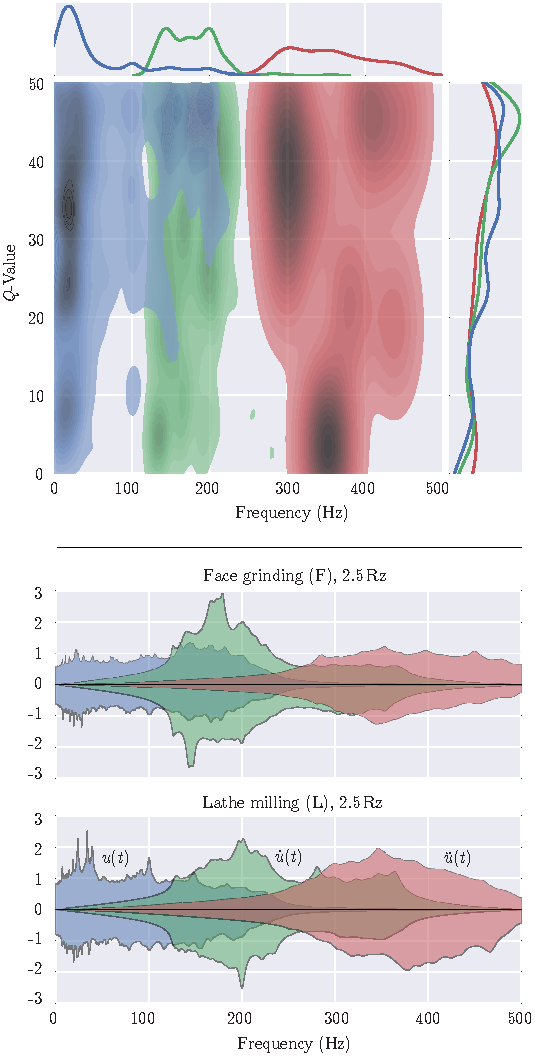
\includegraphics[width=0.4\textwidth]{touch-5}    
    \caption{\label{fig:touch-filters} Visualizing the network in the frequency domain. Frequencies are $0 - 250$, $125 - 375$, or $250 - 500$\,Hz, depending on whether each hidden neuron is encoding a dimension from $u(t)$ (blue), $\dot{u}(t)$ (green), or $\ddot{u}(t)$ (red). (Top) Distribution of bandpass filter parameters from (\ref{eq-bandpass}), weighted by the $\ell^2$-norm of SVM coefficients, and smoothed by a kernel density estimate \cite{michael_waskom_2015_19108}. 
The smallest weights are omitted to reduce visual clutter. Histograms along the sides flatten the distribution across their corresponding axes. (Bottom) Power of bandpass filters per texture (only two shown), weighted by their squared SVM coefficients (unitless). Negatively rectified dimensions are flipped about the $x$-axis for visualization.}
\end{figure}

To evaluate the system, the trained network was tested on each $1$\,s of test data. The 18-dimensional score vector was decoded from the spiking activity of the output population, lowpass filtered with default time constant ($5$\,ms), and sampled every $1$\,ms (see Fig. \ref{fig:touch-raster}). A total score for each texture was obtained by summing together the individual score vectors across the test segment. The classification for each test segment was taken to be the texture with the highest total score. These results are broken down by texture in Table \ref{tab:touch-results}, averaged across each test segment from all four folds, with an overall accuracy of $65.6\%$. The most common classification is the correct texture, in all cases.

By analyzing the trained network, we may succinctly characterize what each classifier is sensitive to in the frequency domain. We visualize this to indicate which bandpass parameters are most important for classifying all textures (see Fig. \ref{fig:touch-filters} top), and which frequencies are most important for classifying a specific texture (see Fig. \ref{fig:touch-filters} bottom). 
The top figure reveals that narrow filters (higher values of $Q$) tend to carry more weight, while frequencies in the range of $50 - 100$, $240 - 260$, and $400 - 500$\,Hz are less useful. The bottom figure shows for example that neurons encoding the negatively rectified dimension of $\dot{u}(t)$ will provide the most evidence for L2.5 when this dimension has power at $200$\,Hz. 

We also compared our approach to a simpler model, 
by training and evaluating the same model without a hidden layer. This baseline model was prepared and validated under the same conditions, except the SVM used the spiking activity of the mechanoreceptor population as its features, rather than the spiking activity from the hidden layer.  Cross-validation accuracy decreased to $17.8\%$, averaged across each test segment from all four folds.
We remark that the baseline still captures temporal information through its various lowpass filters (in the output layer and PSCs) and highpass filters (in the mechanoreceptor cells), yet it is no longer able to isolate particular bands of frequencies. Therefore, it is the addition of bandpass filters in the hidden layer that enable the network to accurately separate the feature space by texture.

\subsubsection{Discussion}

We trained a three-layer network of spiking neurons to classify a set of 18 textures. A biologically plausible model of mechanoreceptors was adapted to encode the input vibrations. Psychophysical experiments and the role of cuneate neurons motivated a hidden layer that extracts frequency information. Lastly, an SVM determined the connection weights into a recurrently connected population. To our knowledge this is a novel semi-supervised approach for classifying dynamic stimuli using a spiking neural network.

A key advantage of our approach is that the network can be simulated in real-time using low-power neuromorphic hardware. At the same time, the NEF endows our model with benefits such as robustness to noise  and parallel computation. Similarly, the system immediately provides classifications online, and performs well with brief inputs lasting only $1$\,s.  These advantages make our method generally suitable for use in robotic applications, thus advancing the state of the art for texture classification. % be more explicit? examples?

A comparison with a baseline model revealed that performance was a consequence of the hidden layer. The first two layers of the network are unsupervised, and so the activity of the hidden layer represents general features that can in theory be reused for other applications. We intend to demonstrate this by extending our system to differentiate between textures, by interpreting the feature vector as a high-dimensional description of a texture. We also suspect that other tasks which process tactile stimuli  can benefit by using this same vector.

Likewise, features of the input stimulus are learned and classified using general techniques from signal processing and machine learning. The methodology that we have described here need not be limited to the use of mechanoreceptor models and bandpass filters. While these tools were needed to appropriately constrain our model, other applications involving the processing of dynamic stimuli (e.g. visual or auditory) may readily place different constraints on how each layer encodes and filters information. This in turn may allow the architecture to be modified and redeployed within other domains. 

The test results indicate how often each texture is confused with another. 
In general, it should be possible to design a simple psychophysical experiment to compare our system to human performance. However, our system is at a fundamental disadvantage since it does not  alter its position or pressure to gather more evidence when unsure of its prediction. We are considering future extensions that solve this issue with a closed-loop system that can actively control its motor movements, with a range of velocities,  based on feedback from the accumulated features.

\subsection{Decoding Filters}

\begin{figure}
\centering
\tikzstyle{block} = [draw, rectangle, minimum height=3em, minimum width=3em]
\tikzstyle{sum} = [draw, circle, node distance=1cm]
\tikzstyle{input} = [coordinate]
\tikzstyle{output} = [coordinate]
\tikzstyle{pinstyle} = [pin edge={to-,thin,black}]
\begin{tikzpicture}[auto, node distance=2cm,>=latex']
  \node [input, name=input] {};
  \node [coordinate, name=fanin, right of=input] {};
  \node [block, right of=fanin, node distance=1cm] (b) {${b}$};
  \node [sum, right of=b, node distance=2cm] (sum) {};
  \node [block, right of=sum, node distance=2cm] (integ) {$H(s)$};
  \node [below of=integ, name=decoded] {$\sum_{i=1}^n a_i(t) {d}_i$};
  \node [output, right of=integ] (output) {};

  \draw [-] (input) -- node {${u}(t)$} (fanin);
  \draw [->] (fanin) -- node {} (b);
  \draw [->] (b) -- node {} (sum);
  \draw [->] (sum) -- node {${w}(t)$} (integ);
  \draw [->] (integ) -- node [name=fanout] {${x}(t)$} (output);
  \draw [->] (decoded) -| node[pos=0.98] {$+$} node [near end] {} (sum);
\end{tikzpicture}
\caption{\label{fig:decoding-filter} Architecture used to formulate an optimization problem that combines the decoding vector with the decoding filter.}
\end{figure}

Here we consider the problem of solving for the optimal linear filter, together with the optimal linear decoders, in the same least-squares optimization problem.
This is useful in the situation where we have freedom over the form of the synaptic filter (e.g., Loihi) and would like to find the best synapse for representing some particular target signal (either feed-forward or recurrently).
We begin by considering the architecture from Fig.~\ref{fig:decoding-filter}.
Beginning with the scalar case, ${x}(t)$ is the known target representation, which here we interpret as the PSC without loss of generality, by moving the filtering to occur before the encoding vector, gain, and bias, by linearity.
$a_i(t)$ is the spike-train of the $i^\text{th}$ neuron encoding ${x}(t)$. ${b}$ is a free parameter scaling the input signal ${u}(t)$. ${d}_i$ are free parameters decoding the activities. Lastly, we'll suppose the synapse has the form:
\begin{equation}
H(s) = \frac{1}{1 + \sum_{i=1}^k c_i s^i} \text{,}
\end{equation}
where $k \in \mathbb{N}_{\ge 1}$ is fixed and $c_i$ ($1 \le i \le k$) are free parameters for the chosen recurrent synapse.
We fix $c_0 = 1$ so that $H(0) = 1 \iff$ its impulse response has an integral of $1$.
\TODO{Reference results on coordinate transformation.}

We define ${w}(t)$ as the signal driving the synapse. Our goal is to satisfy:
\begin{align*}
    && \frac{{X}(s)}{{W}(s)} &= H(s) \\
    \iff && {x}(t) + \sum_{i=1}^k c_i {x}^{(i)}(t) &= {b} \cdot {u}(t) + \sum_{i=1}^n a_i(t) {d}_i \\
    \iff && {b} \cdot {u}(t) + \sum_{i=1}^k c_i \left(-{x}^{(i)}(t)\right) + \sum_{i=1}^n a_i(t) {d}_i &= {x}(t)
\end{align*}

We then rewrite this problem in matrix form $AD = Y$, where:
$$A = \left[ \begin{matrix} {u}(t) & -{x}^{(1)}(t) & \ldots & -{x}^{(k)}(t) & a_1(t) & \ldots & a_n(t)  \end{matrix} \right] \text{,} \quad D = \left[ \begin{matrix} {b} \\ c_1 \\ \vdots \\ c_k \\ d_1 \\ \vdots \\ d_n \end{matrix} \right] \text{,} \quad Y = \left[ \begin{matrix} {x}(t) \end{matrix} \right]\text{,}$$
and each row of $A$ and $Y$ correspond to an evaluation point $t$ from the dataset.

For vector representations, $\V{x}(t)$, we can repeat this independently for each dimension, to solve for a decoding matrix and a vector of synapses. 
Furthermore, if we substitute this target with the desired post-synaptic current, $\alpha_i \left \langle \V{x}(t)\text{,}\, \V{e}_i \right \rangle + \beta_i$---analogous to a core idea from the methods of \citet{stoeckel2018}---then we can repeat this optimization procedure for each neuron to obtain a full weight-matrix and an individual synaptic filter for each neuron, while maintaining the desired encoding.
This can be used to fully leverage hardware where synapses are configurable at the post-synaptic neuron level, in order to improve overall accuracy.

Since our $A$ matrix contains spikes, we should regularize the system by filtering the columns of both $A$ and $Y$ by some filter (e.g.,~lowpass).
Improved accuracy for sparse datasets may be achieved via Generalized Tikhonov regularization, by mapping some Bayesian prior over the poles of $H(s)$\footnote{The time-constants of $h(t)$ are equal to $-p_i^{-1}$ where $p_i$ is the $i^\text{th}$ pole of $H(s)$.} to some corresponding distribution over $c_i$ ($1 \le i \le k$).
This results in a regularization matrix with block-structure, with one block imposing the usual diagonal L2-regularization on the entries corresponding to the $d_i$ parameters, and the other imposing some correlation structure on the $c_i$ parameters given the chosen prior on the unknown time-constants of $h(t)$.

\subsection{Dale's Principle}

Compare my DalesSolver to Parisian Transform

\subsection{Conductance-Based Synapses}

Summarize Andreas' research


\section{Neural Extensions}

\subsection{Poisson Spiking}
\label{sec:poisson-spiking}

In the NEF, there are three sources of error in the neural representation: (1) ``static distortion'' arising from the use of decoders; that is, the linear combination of nonlinear basis functions to approximate some desired transformation, (2) ``spike noise'' arising from the use of discontinuous spikes; that is, the substitution of a continuous non-spiking model with a spiking model that produces variable PSCs, and (3) ``state discrepancy'' arising from the substitution of a stateless model with a stateful model; specifically, when it leads to a violation of the uniform assumption outlined in section~\ref{sec:spike-coding}.

The first two problems can be solved by scaling up the number of neurons.
Static distortion error scales as $\bigoh{n^{-1}}$ in the number of neural basis functions~\citep{eliasmith2003a}.
\TODO{Cite appropriate page in NEF text.}
Spike noise scales as $\bigoh{ \tau^{-1} n^{-1/2} }$.\footnote{The PSC has an amplitude of $\tau^{-1}$ which linearly scales the error $\bigoh{n^{-1/2}}$.}
In this section, we focus on addressing the third source of error, which is independent of the number of neurons.
Furthermore, we address this in the context of Principle~3, where our goal is to precisely compile some set of differential equations onto the spiking network.
In other contexts it may be desirable to leverage stateful behaviour such as adaptation (see section~\ref{sec:adaptive-neurons}) instead of viewing it as a source of error.

As suggested in section~\ref{sec:spike-coding}, the goal is for our neurons to be ``uniformly ready to spike'' at every given moment in time.
The issue with LIF neurons is that, for non-constant inputs, this requirement is systematically violated.
Each neuron is biased away from the median of the distribution, tending towards one of two extremes of either being closer to the start of its ideal ISI or closer to its end (see Fig.~\ref{fig:spike-time-intervals}).
This discrepancy between the true distribution of neural states, and the ideal uniform distribution, worsens as the input frequency increases relative to the spike-rates and time-constants of the neuron model (not shown).
This observation goes well beyond the scope of the LIF model, to any neuron model that has some internal memory or state that leads it to violate the criteria of uniformity.

This discussion motivates the search for a ``memoryless'' spiking neuron model -- one that cannot be biased towards a non-uniform probability of being ready to spike by its prior inputs or absence thereof.
The exponential distribution is the only such continuous-time probability distribution.
This distribution describes the arrival time between Poisson events.
Therefore, a Poisson spiking model is the only probabilistic neuron model that satisfies our criteria for eliminating this source of error.
We thus consider Poisson spiking neurons where the number of spikes within a given time-step follows a Poisson distribution with a rate given by some desired static response curve evaluated at the input current.

Poisson spiking models have numerous benefits.
First, they are cheap to simulate in both space and time, as they require no additional memory or updates to state.
Second, they can be applied to any static response curve without loss of generality.
Third, there is no latency when processing inputs that jump discontinuously, and more generally when processing high-frequency input signals, as there is no start-up transient in the model; the expected spike rate of each neuron always equals the desired instantaneous rate.
Fourth, by solving the state discrepancy problem, the performance continues to scale with the number of neurons.
Fifth, since increasing the input frequency is equivalent to decreasing the spike-rates for a Poisson model, this scaling promotes a reduction in total power by way of fewer spikes needed to achieve some level of precision.

\begin{figure}
\centering
\includegraphics[width=1.0\textwidth]{poisson-frequency-scaling}
\caption{\label{fig:poisson-frequency-scaling} Performance of Poisson LIF versus regular LIF as the frequency of the input signal is scaled.
The input signal is a sinusoid with frequency $f$\,Hz.
Both the ideal sinusoid and the decoded spike trains are filtered by $\tau = 0.01 f^{-1}$\,s to compute the RMSE.
The number of neurons is set to $50 f$ in order to scale the total number of spikes with the input frequency, and the maximum firing rate of each neuron is uniformly distributed over $20-40$\,Hz.
We give the LIF neurons an advantage by washing out the initial transient induced by an initial voltage of $v(0) = 0$.
Due to the variability in the Poisson process, the regular LIF is better for near-constant inputs.
Due to the memoryless property of the Poisson process, the Poisson LIF retains identical performance with higher frequencies.
}
\end{figure}

\begin{figure}
\centering
\includegraphics[width=1.0\textwidth]{poisson-neuron-scaling}
\caption{\label{fig:poisson-neuron-scaling} Performance of Poisson LIF versus regular LIF as the number of neurons are scaled.
The input signal is a sinusoid with frequency $10$\,Hz, and the maximum firing rates are uniformly distributed over $20-40$\,Hz.
Regular LIF plateaus in performance for large numbers of neurons, due to the systematic discrepancy between the neural state and the ideal uniform distribution for non-constant inputs, as shown in section~\ref{sec:spike-coding}.
Poisson LIF performance scales towards $0$ error as $n \rightarrow \infty$, since the memoryless property means each neuron is always ready to spike with the ideal probability. 
}
\end{figure}

We validate these claims in Figure~\ref{fig:poisson-frequency-scaling} and Figure~\ref{fig:poisson-neuron-scaling} by exploring a Poisson spiking version of the LIF model.
These results demonstrate that Poisson spiking models solve the state-discrepancy problem, and thus continue to scale in accuracy with neuron count at increasingly-greater signal frequencies relative to the firing rates.
The properties of this neuron model make it particularly suitable for neuromorphic architectures such as SpiNNaker~2.
Specifically, SpiNNaker~2 has specialized hardware for computing exponentials~\citep{partzsch2017fixed} and uniform samples~\citep{liu2018memory}, and the architecture benefits enormously from the reduction of memory requirements and spike traffic~\citep{mundy2015, stromatias2013power}.
Since the Poisson spike generator can be applied to any desired static response curve, this method can be applied to whatever is cheap to compute while still providing a suitable nonlinear basis for the desired transformation.

\subsection{Adaptative Neurons}
\label{sec:adaptive-neurons}

Partial differentiation (Fairhall)
Eric's system itendification
Subtractive adaptation and perfect cancellation
Divisive adaptation (adaptive threshold) and modelling it by the latter
Interpretation in terms of PSC code / objective function, and dimensionality

\subsection{Wilson Neurons}

Peter's work

\subsection{Baal Neurons}

Peter's work
